\documentclass[12pt, a4paper]{article}

\usepackage[italian]{babel}
\usepackage{geometry}
\usepackage{amsmath}
\usepackage{amssymb}
\usepackage{graphicx}
\usepackage{ulem}
\geometry{margin=1cm}
\usepackage{listings}
\usepackage{xparse}
\usepackage{expl3}
\usepackage{tikz}
\usetikzlibrary{calc}
\let\olditemize\itemize
\renewcommand\itemize{\olditemize\setlength\itemsep{0em}}

\newcommand{\tikzmark}[1]{\tikz[baseline,remember picture] \coordinate (#1) {};}
\newcommand{\bra}[1]{\langle #1 |}
\newcommand{\ket}[1]{| #1 \rangle}
\newcommand{\customfbox}[1]{
    \begin{center}
        \noindent\fbox{\parbox{\dimexpr\linewidth-2\fboxsep-2\fboxrule\relax}{\centering #1}}
    \end{center}
    }
\ExplSyntaxOn
\NewDocumentCommand{\braket}{m O{} m}{ \langle #1 | \tl_if_blank:nTF {#2} {#3} {#2|#3} \rangle }
\ExplSyntaxOff

\title{Relazione Home Assignment 8}
\author{Daniele Sacco (5616921), Daniele Scaffai (5658260), Lorenzo Vaccarecci (5462843)}
\date{}

\begin{document}
\maketitle
\section*{Obiettivo}
L'obiettivo di questo Home Assignment è l'implementazione del protocollo degli errori di Shor, in particolare gli errori di tipo bit flip, phase flip e small error.

\section*{Bit flip}
\section*{Svolgimento}
Abbiamo riprodotto, usando qiskit, il circuito che è stato fornito dal docente. Tra le due barriere viene applicata la porta di Pauli $X$ per simulare il bit flip.
   
\begin{center} 
        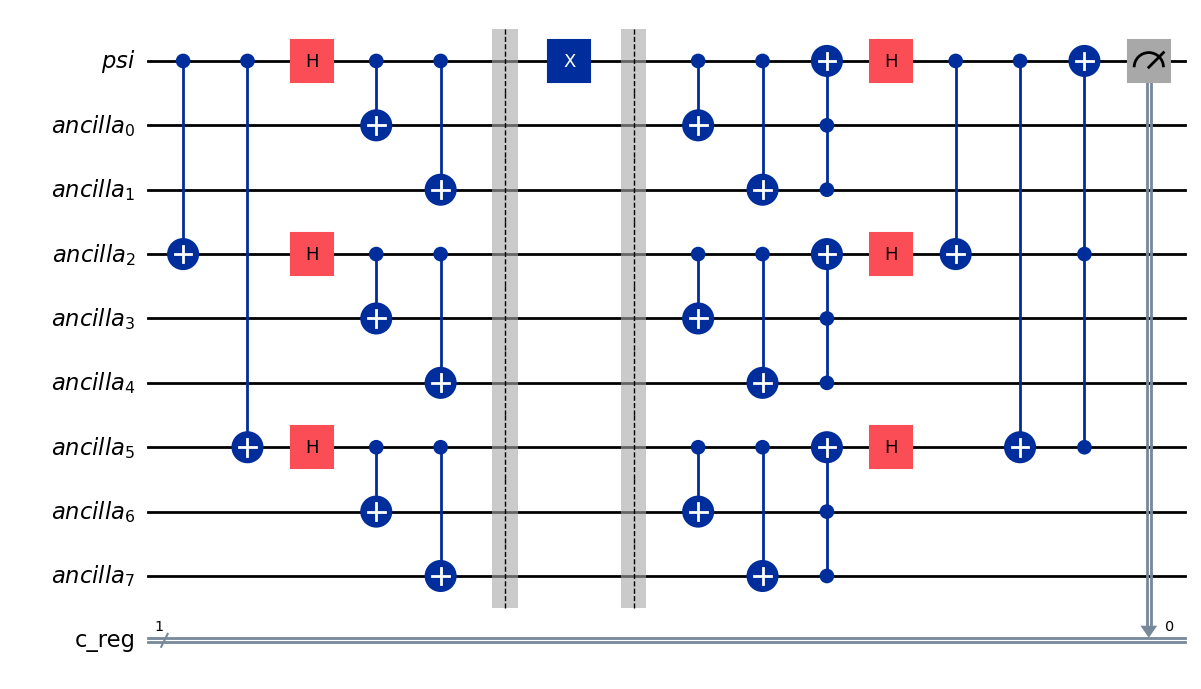
\includegraphics[width=0.6\textwidth]{img/circuit.png} 
        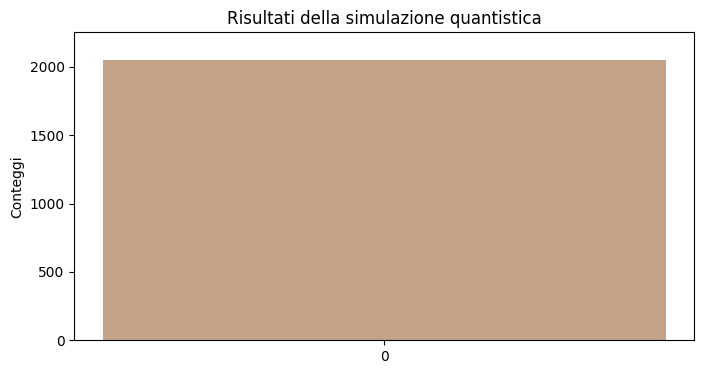
\includegraphics[width=0.4\textwidth]{img/resultsSuccess.png}
\end{center}

\section*{Phase flip}
\section*{Svolgimento}
Abbiamo riprodotto, usando qiskit, il circuito che è stato fornito dal docente. Tra le due barriere viene applicata la porta di Pauli $Z$ per simulare il phase flip.
   
\begin{center} 
        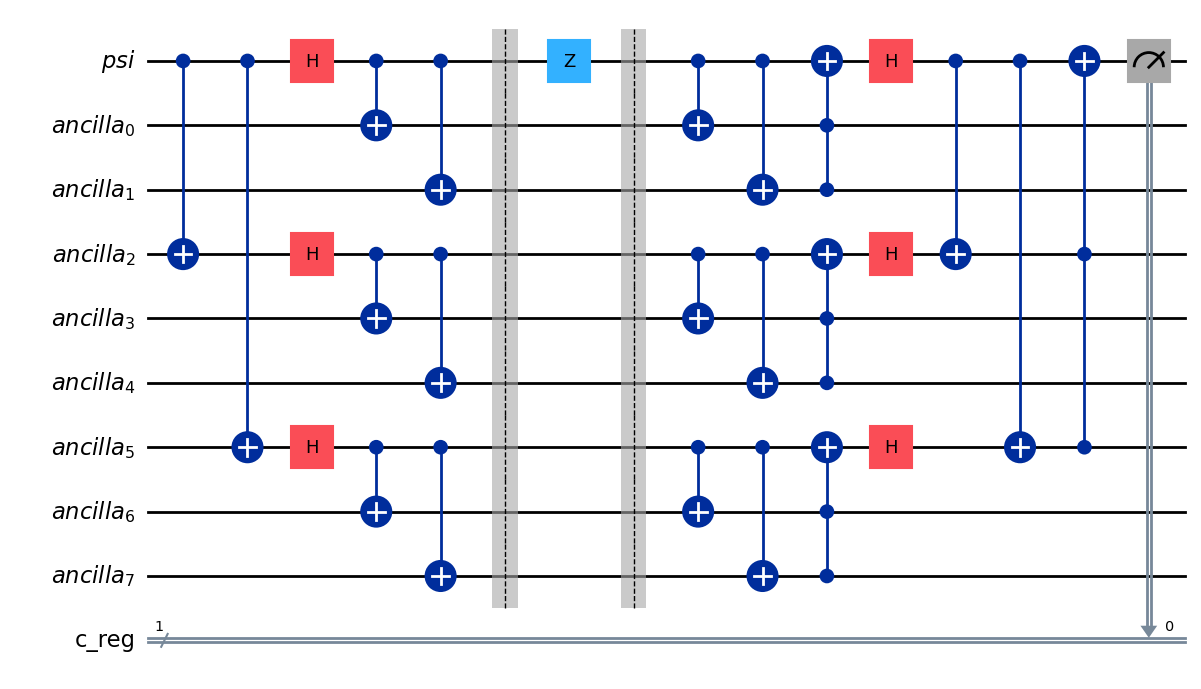
\includegraphics[width=0.6\textwidth]{img/circuitPhaseflip.png} 
        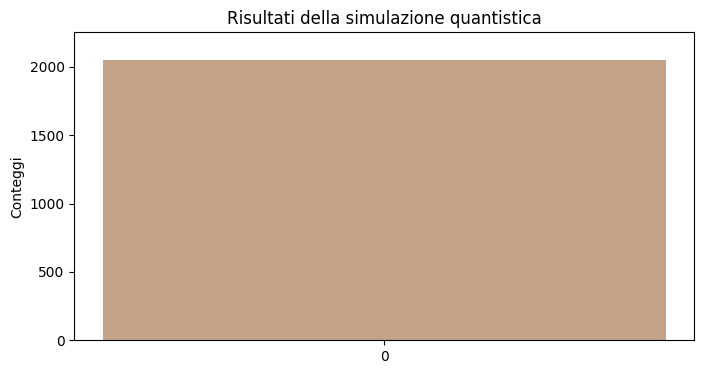
\includegraphics[width=0.4\textwidth]{img/resultsSuccessPhaseflip.png}
\end{center}

\section*{Small error}
\section*{Svolgimento}
Abbiamo riprodotto, usando qiskit, il circuito che è stato fornito dal docente. Tra le due barriere viene applicata una piccola rotazione sull'asse delle $x$ a $\ket{\psi}$ per simulare uno small error.
   
\begin{center} 
        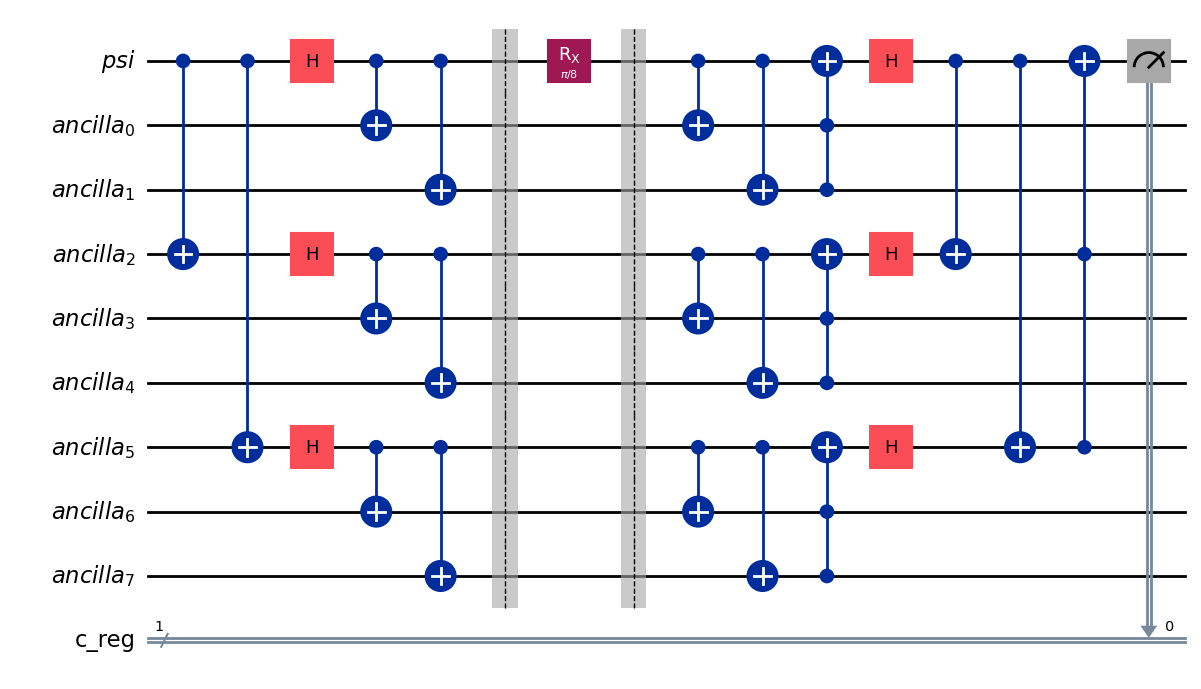
\includegraphics[width=0.6\textwidth]{img/circuitSmallError.png} 
        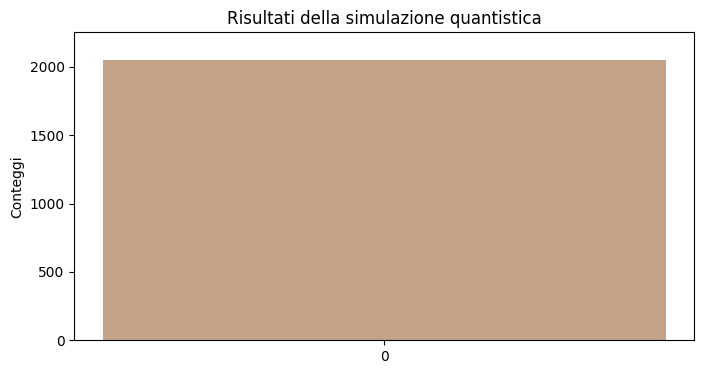
\includegraphics[width=0.4\textwidth]{img/resultsSuccessSmallError.png}
\end{center}

\section*{Risultati}
E' stato aggiunto un misuratore alla fine di ogni circuito e sono state eseguite 2048 simulazioni per ciascuno. La misura attesa per ogni tipo di errore è 0, perchè è lo stato iniziale di $\ket{\psi}$.

\section*{Conclusioni}
I risultati ottenuti corrispondono a quelli attesi, quindi possiamo concludere che l'implementazione del protocollo di correzione degli errori di Shor è corretta.

\end{document}